\documentclass{article}
\usepackage{amsmath} % import of math elements
%\usepackage{mathtools} %import of other math elements
\usepackage{tikz} 
\usetikzlibrary{shapes,positioning,calc} 
\usetikzlibrary{positioning,matrix, arrows.meta}
\usetikzlibrary{decorations.pathreplacing}
\usepackage{listings}
\usepackage{color}
\definecolor{dkgreen}{rgb}{0,0.6,0}
\definecolor{gray}{rgb}{0.5,0.5,0.5}
\definecolor{mauve}{rgb}{0.58,0,0.82}

\lstset{frame=tb,
  language=Bash,
  aboveskip=3mm,
  belowskip=3mm,
  showstringspaces=false,
  columns=flexible,
  basicstyle={\small\ttfamily},
  numbers=none,
  numberstyle=\tiny\color{gray},
  keywordstyle=\color{blue},
  commentstyle=\color{dkgreen},
  stringstyle=\color{mauve},
  breaklines=true,
  breakatwhitespace=true,
  tabsize=3
}

%-------------------------------------------------------
% Document information
%-------------------------------------------------------

\title{Algorithm and data structures} %Title 

\author{Roberto \textsc{Antoniello}} %author name

\begin{document}
\maketitle % show the title and author and date
%-------------------------------------------------------
%Introduction
%-------------------------------------------------------

\begin{center} In this file I will resume all the concepts I liked while studying the course of Algorithm and data structures.\end{center}

\section{Binary search}
This algorithm can be used only if you have a sorted array. Here how it works: \\
BinarySearch take a sorted array as input and return an index as output. So it returns the index of the found element or -1 if not found.\\
When it starts execution, the algorithm saves three variables \textbf{sx}, \textbf{dx} and \textbf{m}. The \textbf{m} variable is the index in the middle of the array, \textbf{sx} and \textbf{dx} are the first and the last index. It asks if the element is less or more than the element in \textbf{m} position. \\
Basically, if the element is x the question is: 
\textbf{x $<$ A[m]}  or  \textbf{x $>$ A[m]} ? 
We are reducing the search space by 2 every time because if it's less, our \textbf{dx} becomes \textbf{m}, otherwise our \textbf{sx} becomes \textbf{m+1}. \\
At the first iteration the search space is n elements, at the second it is $\cfrac{n}{2}$, at the third one it is $\cfrac{n}{2^2}$ and so on.\\
At the i° iteration it will be $\cfrac{n}{2^i}$.\\
During the last iteration the size of our array A is 1. So:\\
$\cfrac{n}{2^i} = 1 \Rightarrow n = 2^i \Rightarrow i = \log_2{n}$ \\
We have just said the amount of steps are $\log_2{n} \Rightarrow O(\log{n})$ \\
Here below there's an array as example with the initial value of sx,m and dx. \\

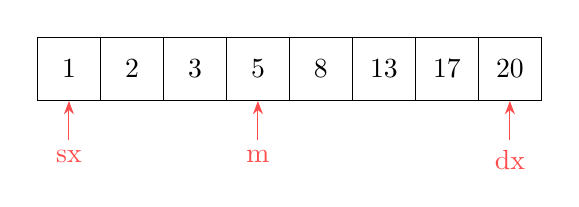
\begin{tikzpicture}
    \matrix (A) [matrix of nodes, nodes={draw, minimum size=8mm},
    column sep=-\pgflinewidth]{
        1 & 2 & 3 & 5 & 8 & 13 & 17 & 20\\
    };

    \foreach \i [evaluate=\i as \ni using {int(\i)},] in {1, 4, 8}{
        \pgfmathtruncatemacro{\half}{(\i + 1) / 2}
        \ifnum \i = 1
            \def\arrowlabel{sx}
        \else
            \ifnum \i = 4
                \def\arrowlabel{m}
            \else
                \def\arrowlabel{dx}
            \fi
        \fi
        \draw [{Stealth}-, red!70] (A-1-\ni.south) -- ++(-90:5mm) node[below] {\arrowlabel};
    }
\end{tikzpicture}

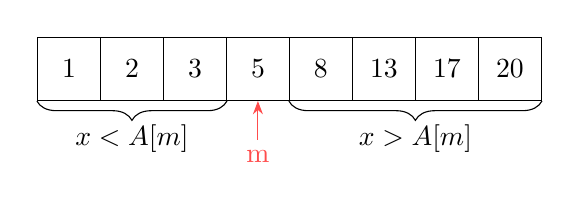
\begin{tikzpicture}
    \matrix (A) [matrix of nodes, nodes={draw, minimum size=8mm},
    column sep=-\pgflinewidth]{
        1 & 2 & 3 & 5 & 8 & 13 & 17 & 20\\
    };

    \foreach \i [evaluate=\i as \ni using {int(\i)},] in {4}{
        \pgfmathtruncatemacro{\half}{(\i + 1) / 2}
        \ifnum \i = 4
        		\def\arrowlabel{m}
        	\fi
        \draw [{Stealth}-, red!70] (A-1-\ni.south) -- ++(-90:5mm) node[below] {\arrowlabel};
    }

    % Brace for x < A[m]
    \draw [decorate,decoration={brace,amplitude=7pt,mirror},xshift=-1pt,yshift=-2pt]
        (A-1-1.south west) -- (A-1-3.south east) node[midway,below=5pt] {${x < A[m]}$};

    % Brace for x > A[m]
    \draw [decorate,decoration={brace,amplitude=7pt,mirror},xshift=-1pt,yshift=-2pt]
        (A-1-5.south west) -- (A-1-8.south east) node[midway,below=5pt] {${x > A[m]}$};
\end{tikzpicture}


I let you read the pseudocode here below. \\ \\ \\

\begin{lstlisting}[caption={\\\textit{Iterative version of the binary search algorithm.}}]
Algorithm BinarySearch(Array A[0,..,n-1]) --> index
	sx <-- 0
	dx <-- n
	index <-- -1
	while sx < dx do
		m <-- (sx+dx) / 2
		if x < A[m] then
			dx <-- m
		else if x = A[m] then
			index <-- m
		else
			sx <-- m+1
\end{lstlisting}

\section{Selection Sort}
So we know that to do a biinary search, we need a sorted array. \\
There are many solutions to sort an array with more or less complexity in time and space. \\
The first algorithm we're gonna see is the selection sort. This sorting algorithm is really simple, essentially it slides the array and when it find the minimum value it put it at the beginning in the right place. After this step we consider that element sorted and so on until we have the entire array sorted. \\
Let's see here below the pseudocode and then a quick and easy complexity analysis. \\

\begin{lstlisting}[caption={\\\textit{Selection sort algorithm.}}]
Algorithm SelectionSort(Array A[0,..,n-1]) 
	for k <-- 1 to n-2 do
		//finding the index m of minimum value between k and n-1
		m <-- k
		for j <-- k+1 to n-1 do
			if A[j] < A[m] then
				m <-- j
		swap A[m] with A[k]
\end{lstlisting}
The first for cycle ends at \textbf{n-2} because the last element is already sorted if we remember how it works the algorithm. \\
The second for cycle finds the minimum value starting from m position.\\
So, how many comparisons have I to do?\\
If we look at our array A, we can consider that at the k iteration we have \textbf{k} sorted elements on the left and \textbf{n-k-1} to sort on the right.\\

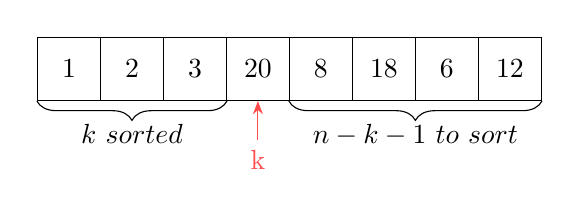
\begin{tikzpicture}
    \matrix (A) [matrix of nodes, nodes={draw, minimum size=8mm},
    column sep=-\pgflinewidth]{
        1 & 2 & 3 & 20 & 8 & 18 & 6 & 12\\
    };

    \foreach \i [evaluate=\i as \ni using {int(\i)},] in {4}{
        \pgfmathtruncatemacro{\half}{(\i + 1) / 2}
        \ifnum \i = 4
        		\def\arrowlabel{k}
        	\fi
        \draw [{Stealth}-, red!70] (A-1-\ni.south) -- ++(-90:5mm) node[below] {\arrowlabel};
    }

    % Brace for x < A[m]
    \draw [decorate,decoration={brace,amplitude=7pt,mirror},xshift=-1pt,yshift=-2pt]
        (A-1-1.south west) -- (A-1-3.south east) node[midway,below=5pt] {${k \ sorted}$};

    % Brace for x > A[m]
    \draw [decorate,decoration={brace,amplitude=7pt,mirror},xshift=-1pt,yshift=-2pt]
        (A-1-5.south west) -- (A-1-8.south east) node[midway,below=5pt] {${n-k-1 \ to \ sort}$};
\end{tikzpicture}
 
 Basically we are doing this sum: \\
 $$\sum_{k=0}^{n-2}(n-k-1)$$
This is equal to sum every $n \in \mathcal{N}$ from 0 to n-2, so:\\
$$\sum_{k=0}^{n-2}(n-k-1) = \sum_{i=1}^{n+1} i = \cfrac{n \cdot (n-1)}{2}$$
This is the total of comparisons I have to do in this algorithm.
The complexity is thus $\Theta(n^2)$. \\
We can say also that this amount of comparisons is always done because we do not set any condition to do these comparisons.

\section{Bubble sort}
The second sorting algorithm we're gonna see is Bubble sort.\\
This works by sliding the array and compare the current element with the previous one. The bigger element is moved in the next position. This make the bigger element go forward until there's another bigger than it. It's called bubble because these big values go forward like the bubbles in the water.\\
Let's do a simulation here below.\\

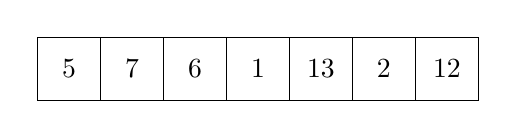
\begin{tikzpicture}
    \matrix (A) [matrix of nodes, nodes={draw, minimum size=8mm},
    column sep=-\pgflinewidth]{
        5 & 7 & 6 & 1 & 13 & 2 & 12\\
    };
\end{tikzpicture}

let's do the first iteration.\\

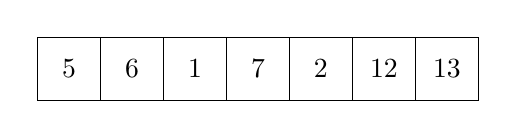
\begin{tikzpicture}
    \matrix (A) [matrix of nodes, nodes={draw, minimum size=8mm},
    column sep=-\pgflinewidth]{
        5 & 6 & 1 & 7 & 2 & 12 & 13\\
    };
\end{tikzpicture}


\begin{center}We compared 5 with 7 $\Rightarrow$ already sorted. \\
Then 7 with 6 $\Rightarrow$ swap. \\
Then 7 with 1 $\Rightarrow$ swap. \\
Then 7 with 13 $\Rightarrow$ already sorted. \\
Then 13 with 2 $\Rightarrow$ swap. \\
Then 13 with 12 $\Rightarrow$ swap. \\

In the next iteration I'll slide again until the entire array is sorted.\\ \end{center}

Now we consider the pseudocode.\\

\begin{lstlisting}[caption={\\\textit{Bubble sort algorithm.}}]
Algorithm BubbleSort(Array A[0,..,n-1]) 
	i <-- 1
	do
		swapped <-- false
		for j <--1 to n-i do
			if A[j] < A[j-1] then
				swap A[j] with A[j-1]
				swapped <-- true
		i <-- i + 1
	while swapped and i < n	
\end{lstlisting}

The for cycle ends at \textbf{n-i} because the last \textbf{i} elements are already sorted as we discussed how it work bubble sort. The external do while cycle ends when we did an iteration without any swap of elements or we reached the \textbf{n-1} iteration. The \textbf{i $<$ n} condition saves us the last iteration without any swap sliding the already sorted array.\\
Let's analyse the comparisons. Inside the main for cycle we do \textbf{n-i} comparisons where \textbf{i} starts at \textbf{1} to \textbf{n-1}. We're doing this sum:\\
$$\sum_{i=1}^{n-1}(n-i) = \sum_{k=1}^{n-1}k = \cfrac{n \cdot (n+1)}{2} = \Theta(n^2)$$
Again, the total amount of comparisons is in the order of $n^2$, but there's a difference between selection sort and bubble sort. That's because here we have this amount of comparisons only in the worst case(reverse sorted array), but in the best case(array already sorted) we can easily see that the amount of comparisons is in the order of $\Theta(n)$ because we just slide one time the array and then the algorithm ends doing \textbf{n-1} comparisons.

\section{Merge sort}
Let's consider the idea of having two already sorted arrays.\\
How can we build an array that contains all the elements sorted?\\
The first option we can think is to do a bubble sort and surely we can do it in $n^2$ steps. \\
Anyway there's a clever way to do this and it's called \textbf{merge}.

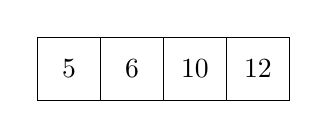
\begin{tikzpicture}
    \matrix (A) [matrix of nodes, nodes={draw, minimum size=8mm},
    column sep=-\pgflinewidth]{
        5 & 6 & 10 & 12 \\
    };
\end{tikzpicture}
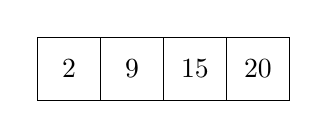
\begin{tikzpicture}
    \matrix (A) [matrix of nodes, nodes={draw, minimum size=8mm},
    column sep=-\pgflinewidth]{
         2 & 9 & 15 & 20\\
    };
\end{tikzpicture}

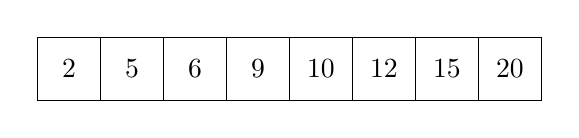
\begin{tikzpicture}
    \matrix (A) [matrix of nodes, nodes={draw, minimum size=8mm},
    column sep=-\pgflinewidth]{
         2 & 5 & 6 & 9 & 10 & 12 & 15 & 20\\
    };
\end{tikzpicture}

The merge procedure works as this: \\
at every step I compare the first two numbers and the mininum go in the final array. When one of the sorted array ends, I append the remaining numbers of the other array without compare anything.\\
How much it costs? Well, every compare will put an element in the right place, so in the worst case I compare all the elements and the remaining is only one element in the other array. So the merge procedure has complexity in the order of $O(n)$ because I do \textbf{n-1} comparisons in the worst case.\\
Here below I drop the pseudocode of a simple version of the merge procedure, which it isn't perfectly optimized in memory.\\


\end{document}
